\documentclass[11pt]{article}
\usepackage[utf8]{inputenc} % Para caracteres en espa�ol
\usepackage{amsmath,amsthm,amsfonts,amssymb,amscd}
\usepackage{multirow,booktabs}
\usepackage[table]{xcolor}
\usepackage{fullpage}
\usepackage{lastpage}
\usepackage{enumitem}
\usepackage{multicol}
\usepackage{fancyhdr}
\usepackage{mathrsfs}
\usepackage{pdfpages}
\usepackage{wrapfig}
\usepackage{setspace}
\usepackage{esvect}
\usepackage{calc}
\usepackage{multicol}
\usepackage{cancel}
\usepackage{graphicx}
\graphicspath{ {pictures/} }
\usepackage[retainorgcmds]{IEEEtrantools}
\usepackage[margin=3cm]{geometry}
\usepackage{amsmath}
\newlength{\tabcont}
\setlength{\parindent}{0.0in}
\setlength{\parskip}{0.05in}
\usepackage{empheq}
\usepackage{framed}
\usepackage[most]{tcolorbox}
\usepackage{xcolor}
\colorlet{shadecolor}{orange!15}
\parindent 0in
\parskip 12pt
\geometry{margin=1in, headsep=0.25in}
\theoremstyle{definition}
\newtheorem{defn}{Definition}
\newtheorem{reg}{Rule}
\newtheorem{exer}{Exercise}

% Two more packages that make it easy to show MATLAB code
\usepackage[T1]{fontenc}
\usepackage[framed,numbered]{matlab-prettifier}
\lstset{
	style = Matlab-editor,
	basicstyle=\mlttfamily\small,
}

\newtheorem{note}{Note}
\begin{document}
\setcounter{section}{0}

\thispagestyle{empty}

\begin{center}
{\LARGE \bf Homework 4}\\
{\large AE453 - Spring 2018 \\ Emilio R. Gordon}
\end{center}
\section*{Problem 1:}
\begin{figure}[H]
\begin{lstlisting}
function hw4p1
t = [0:1:250]/1000; i=1; dzdt = 0; z = 0; V = 0;

while i<1+length(t)
    if i<100
        dzdt = [dzdt 2];
        z = [z zloc(dzdt(i),t(i))];
        V = [V Vz(dzdt(i),z(i))];
    elseif (i>100)&(i<151)
        dzdt = [dzdt 0];
        z = [z zloc(dzdt(100),t(100))+zloc(dzdt(i),t(i))];
        V = [V Vz(dzdt(i),z(i))];
    elseif i>150
        dzdt = [dzdt -2];
        z(150)
        zloc(dzdt(i),t(i))
        z = [z z(150)+zloc(dzdt(i),(t(i)-.15))];
        V = [V Vz(dzdt(i),z(i))];
    end
    i=i+1;
end
figure(1)
plot(t*1000,V,'LineWidth',2)

AxialDistance = [0:.0002:.200]
for j=1:length(AxialDistance)
        VV(1,j)=Vz(2,AxialDistance(j));
        VV(2,j)=Vz(-2,AxialDistance(j));
end
figure(2)
plot(AxialDistance*1000,VV(1,:),'-b','LineWidth',2)
hold on
plot(AxialDistance*1000,VV(2,:),'-r','LineWidth',2)
%Plotting code removed for space. Please see Github for full code.
end

function V = Vz(dzdt,z)
    n = 50;
    A = 1.963e-5;
    mu = 1.256e-6;
    JN = 100;
    a = 0.05;
    Constant1 = ((n*A*3*mu*JN*a^2)/2)*dzdt;
    V = Constant1*(z/((a^2+z^2)^(5/2)));
end

function z = zloc(dzdt,t)
    z = dzdt*t;
end
\end{lstlisting}
\caption{Problem 1: Voltage Trace Code}
\end{figure}
\newpage
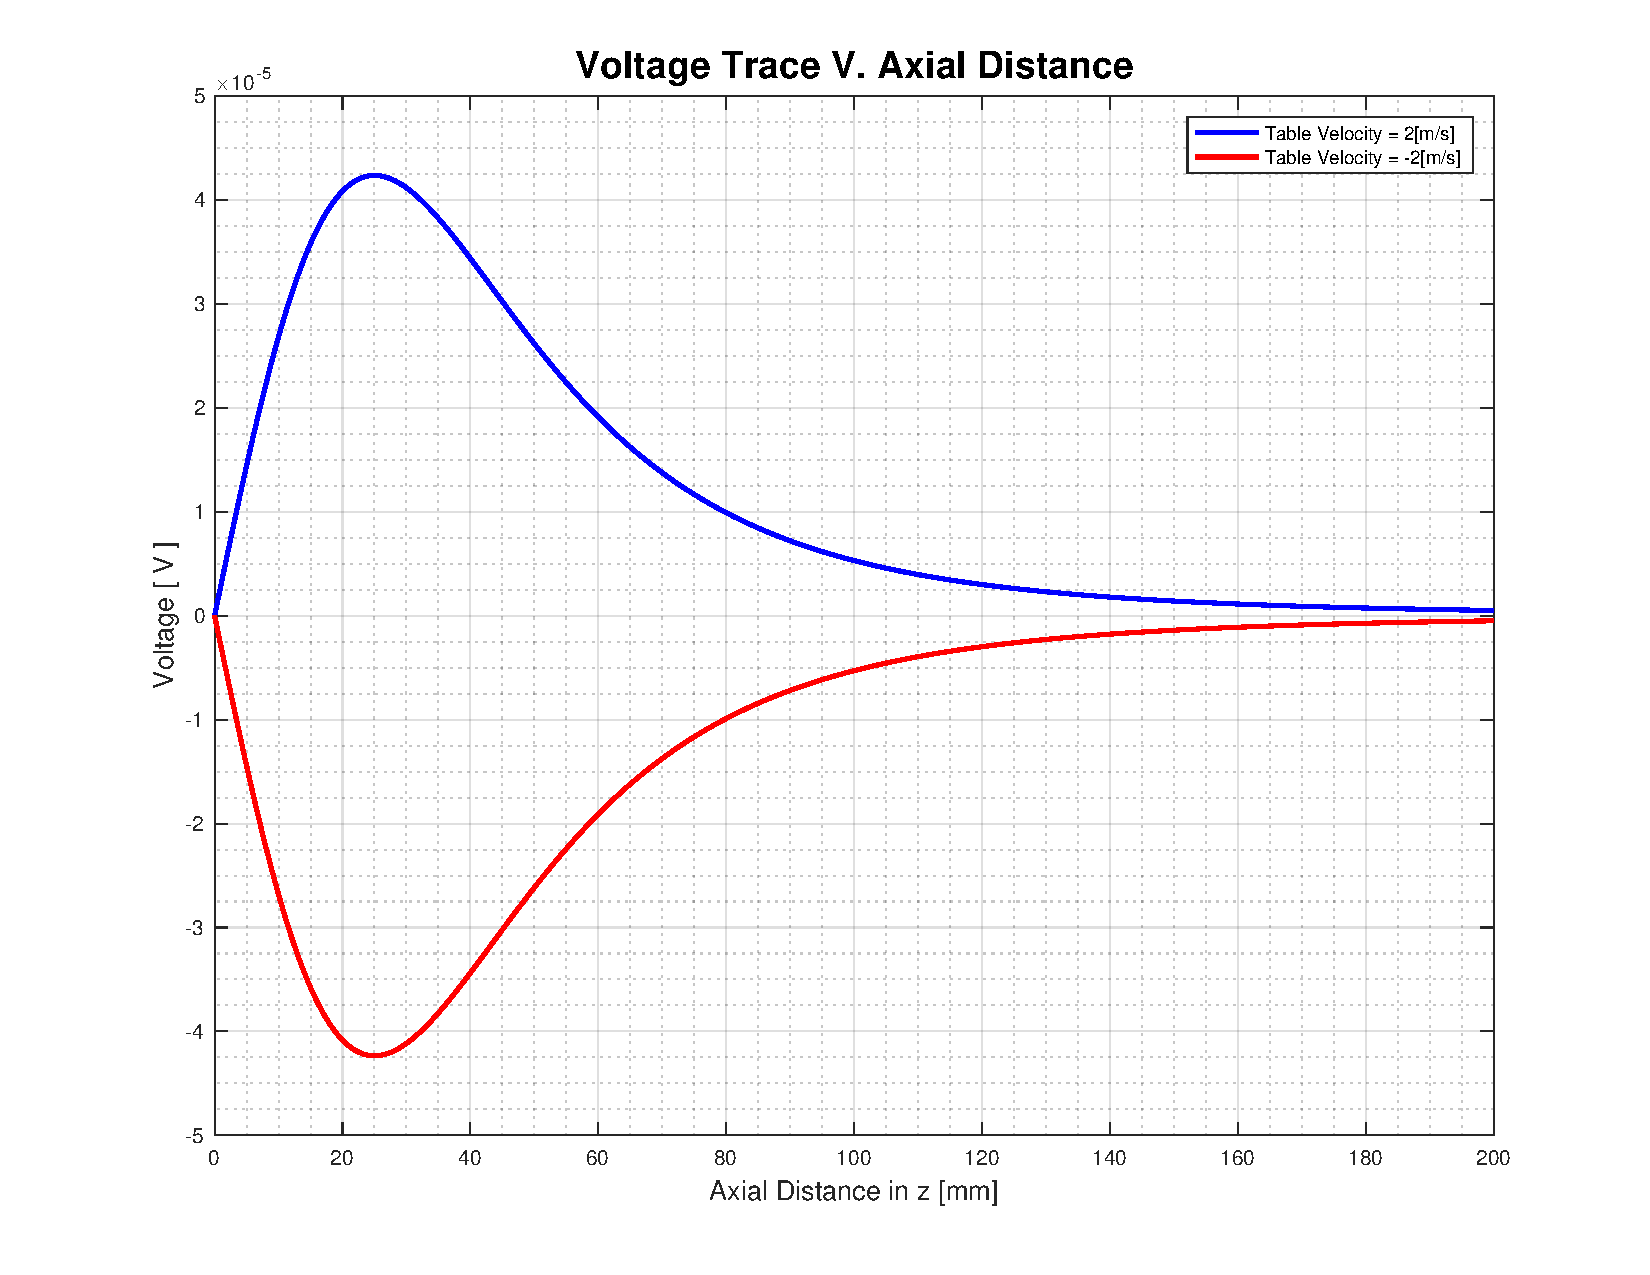
\includepdf{Problem1VoltageVDistance.pdf}
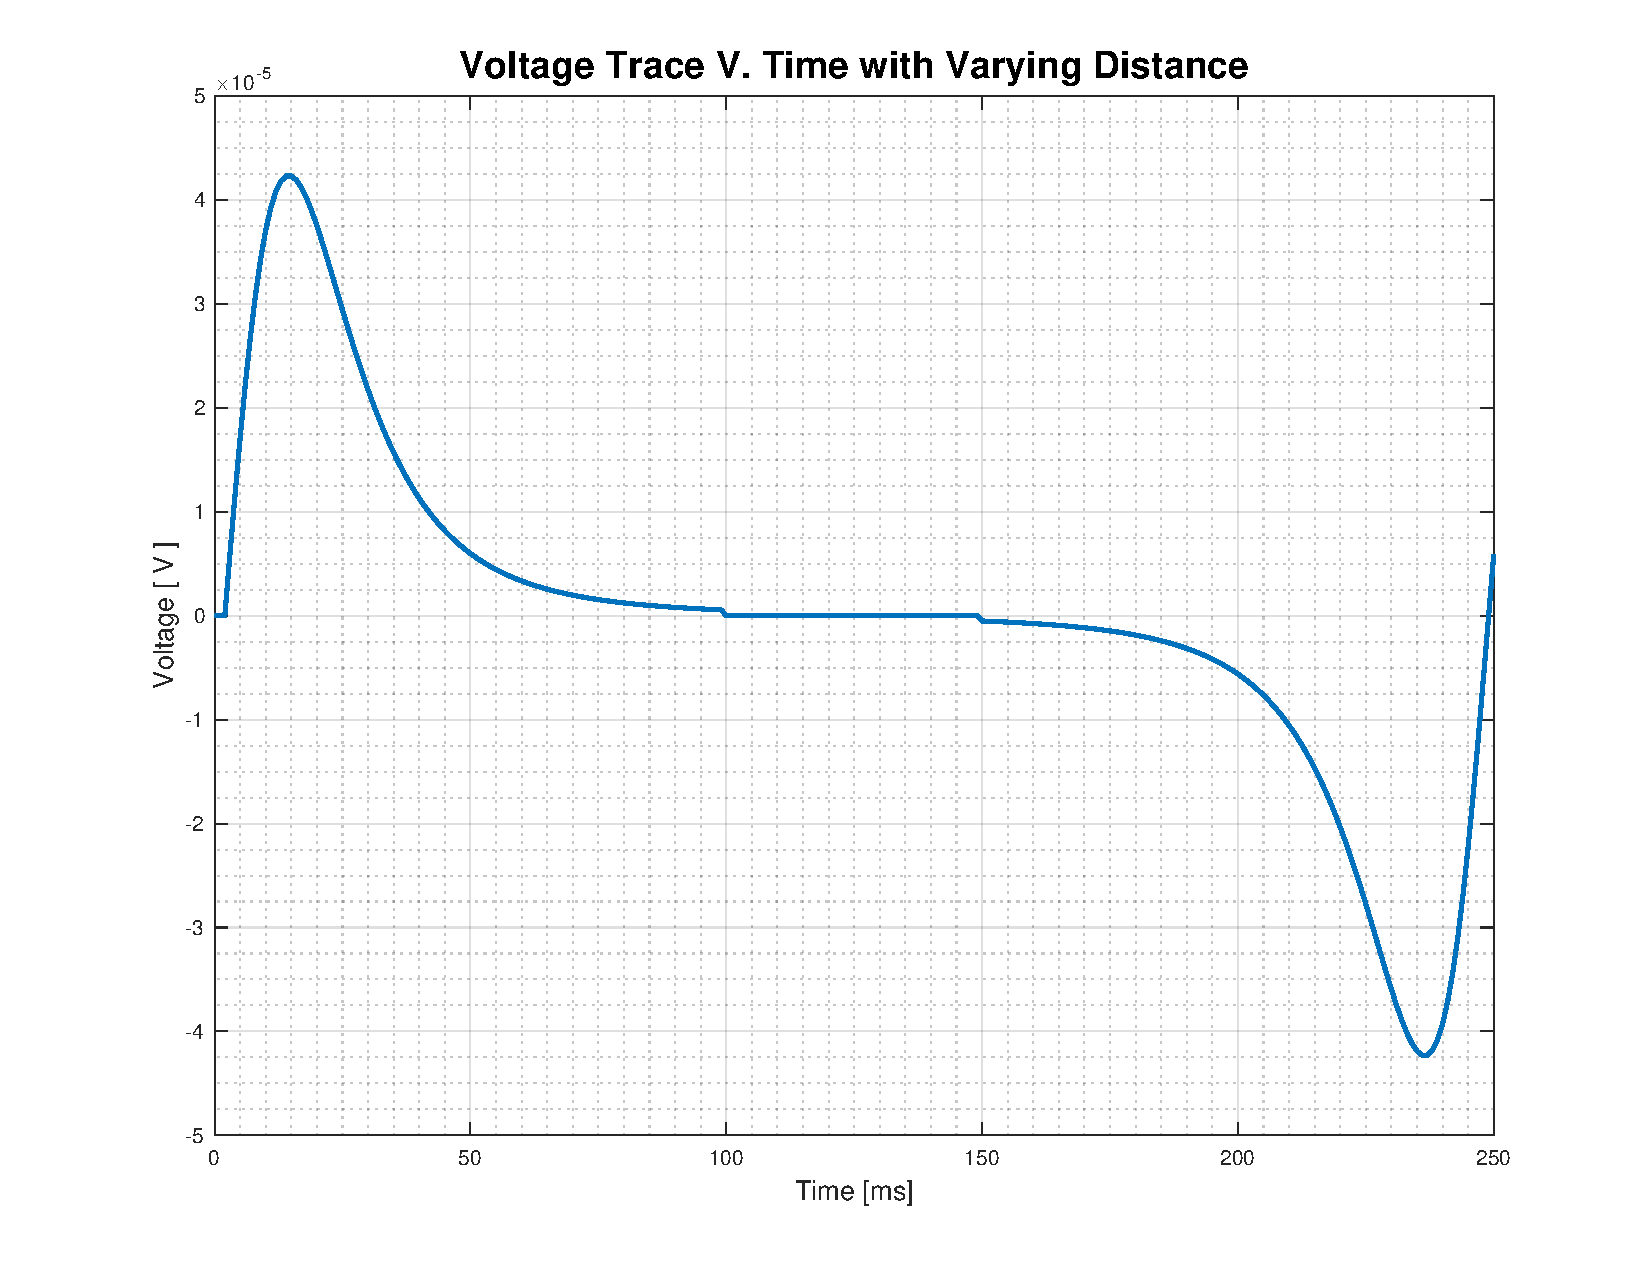
\includepdf{Problem1VoltageVTime.pdf}

\section*{Problem 3: Electron}
\begin{figure}[H]
\begin{lstlisting}
clc; clear;

% Initialize variables
m = 4.48e-26;     % Mass of Electron [kg]
k = 1.38e-23;     % Boltzmann's constant [J/K]
Te = [5; 50];           % Particle Temperature [eV]

% Convert eV to K
T = 1.16045221e4*Te; %Temperature [K]

% Compute two frequently used constants
C1 = [4*pi*(m/(2*pi*k*T(1)))^(3/2);4*pi*(m/(2*pi*k*T(2)))^(3/2);]
C2 = [m/(2*k*T(1));m/(2*k*T(2))];
C3 = [(m/(2*pi*k*T(1)))^(1/2);(m/(2*pi*k*T(2)))^(1/2)];

c_mp1 = sqrt((2*k*T(1))/(m)) %Most Probable Speed
c_mp2 = sqrt((2*k*T(2))/(m))

c = [-3*c_mp2:50:3*c_mp2];  % Particle Velocity Magnitude [m/s]
for i=1:length(c)
    %Maxwellian Speed Distribution Function
    if c(i)<0
        chiM(1,i)=0;
        chiM(2,i)=0;
    else
        chiM(1,i) = C1(1) * c(i)^2 * exp(-C2(1) * c(i)^2);
        chiM(2,i) = C1(2) * c(i)^2 * exp(-C2(2) * c(i)^2);
    end
    
    %Maxwellian Velocity Distribution Function
    fM(1,i) = C3(1) * exp(-C2(1) * c(i)^2);
    fM(2,i) = C3(2) * exp(-C2(2) * c(i)^2);
end

hold on
plot(c/c_mp1,chiM(1,:)*c_mp1,'-b','LineWidth',2) %normalize with cmp.
plot(c/c_mp1,chiM(2,:)*c_mp1,'-r','LineWidth',2) %normalize with cmp.
plot(c/c_mp1,fM(1,:)*c_mp1,'--b','LineWidth',2)
plot(c/c_mp1,fM(2,:)*c_mp1,'--r','LineWidth',2)
hold off

subplot(2,1,1)
hold on
plot(c/c_mp1,chiM(1,:)*c_mp1,'-b','LineWidth',2) %normalize with cmp.
plot(c/c_mp1,fM(1,:)*c_mp1,'--b','LineWidth',2)
hold off
subplot(2,1,2)
hold on
plot(c/c_mp2,fM(2,:)*c_mp2,'--r','LineWidth',2)
plot(c/c_mp2,chiM(2,:)*c_mp2,'-r','LineWidth',2) %normalize with cmp.
\end{lstlisting}
\caption{Problem 3: Normalized Velocity and Speed Distribution Function Code for Electron}
\end{figure}
\newpage
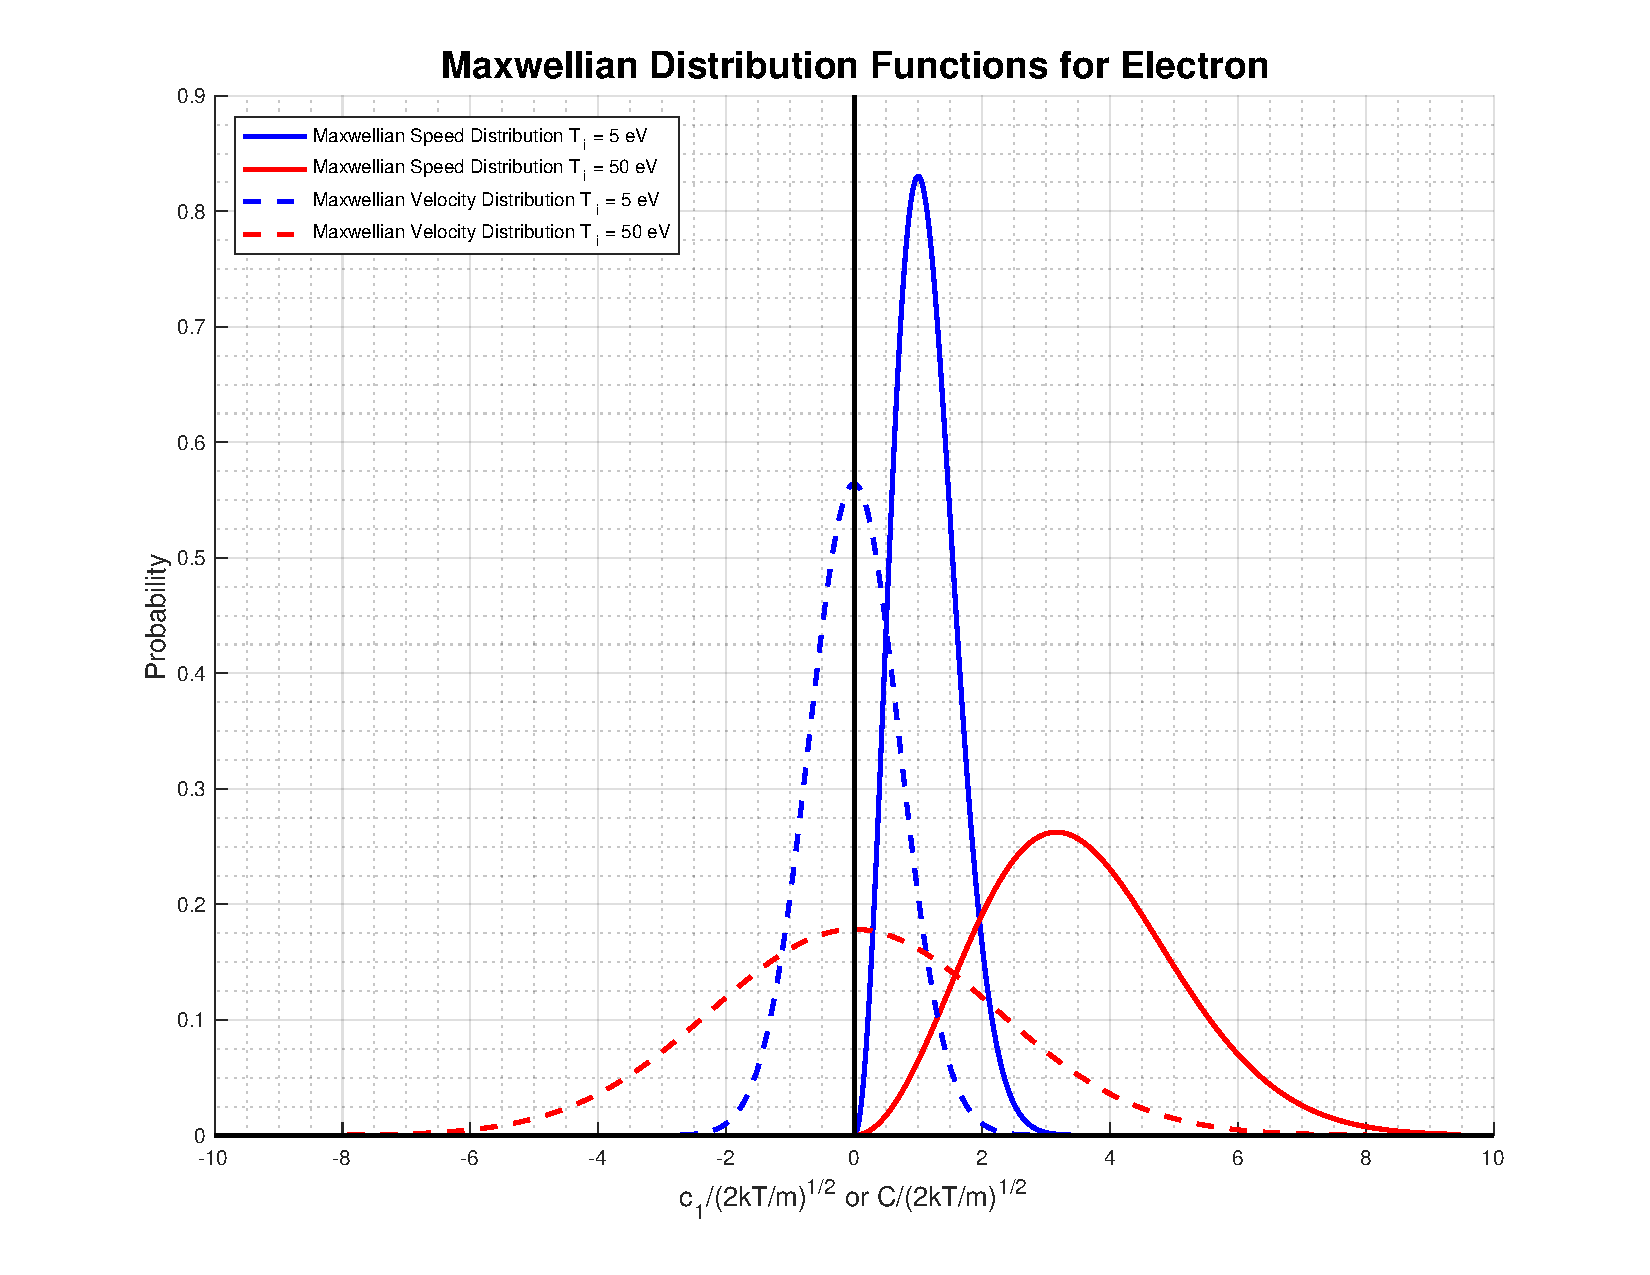
\includepdf{electronBoth.pdf}
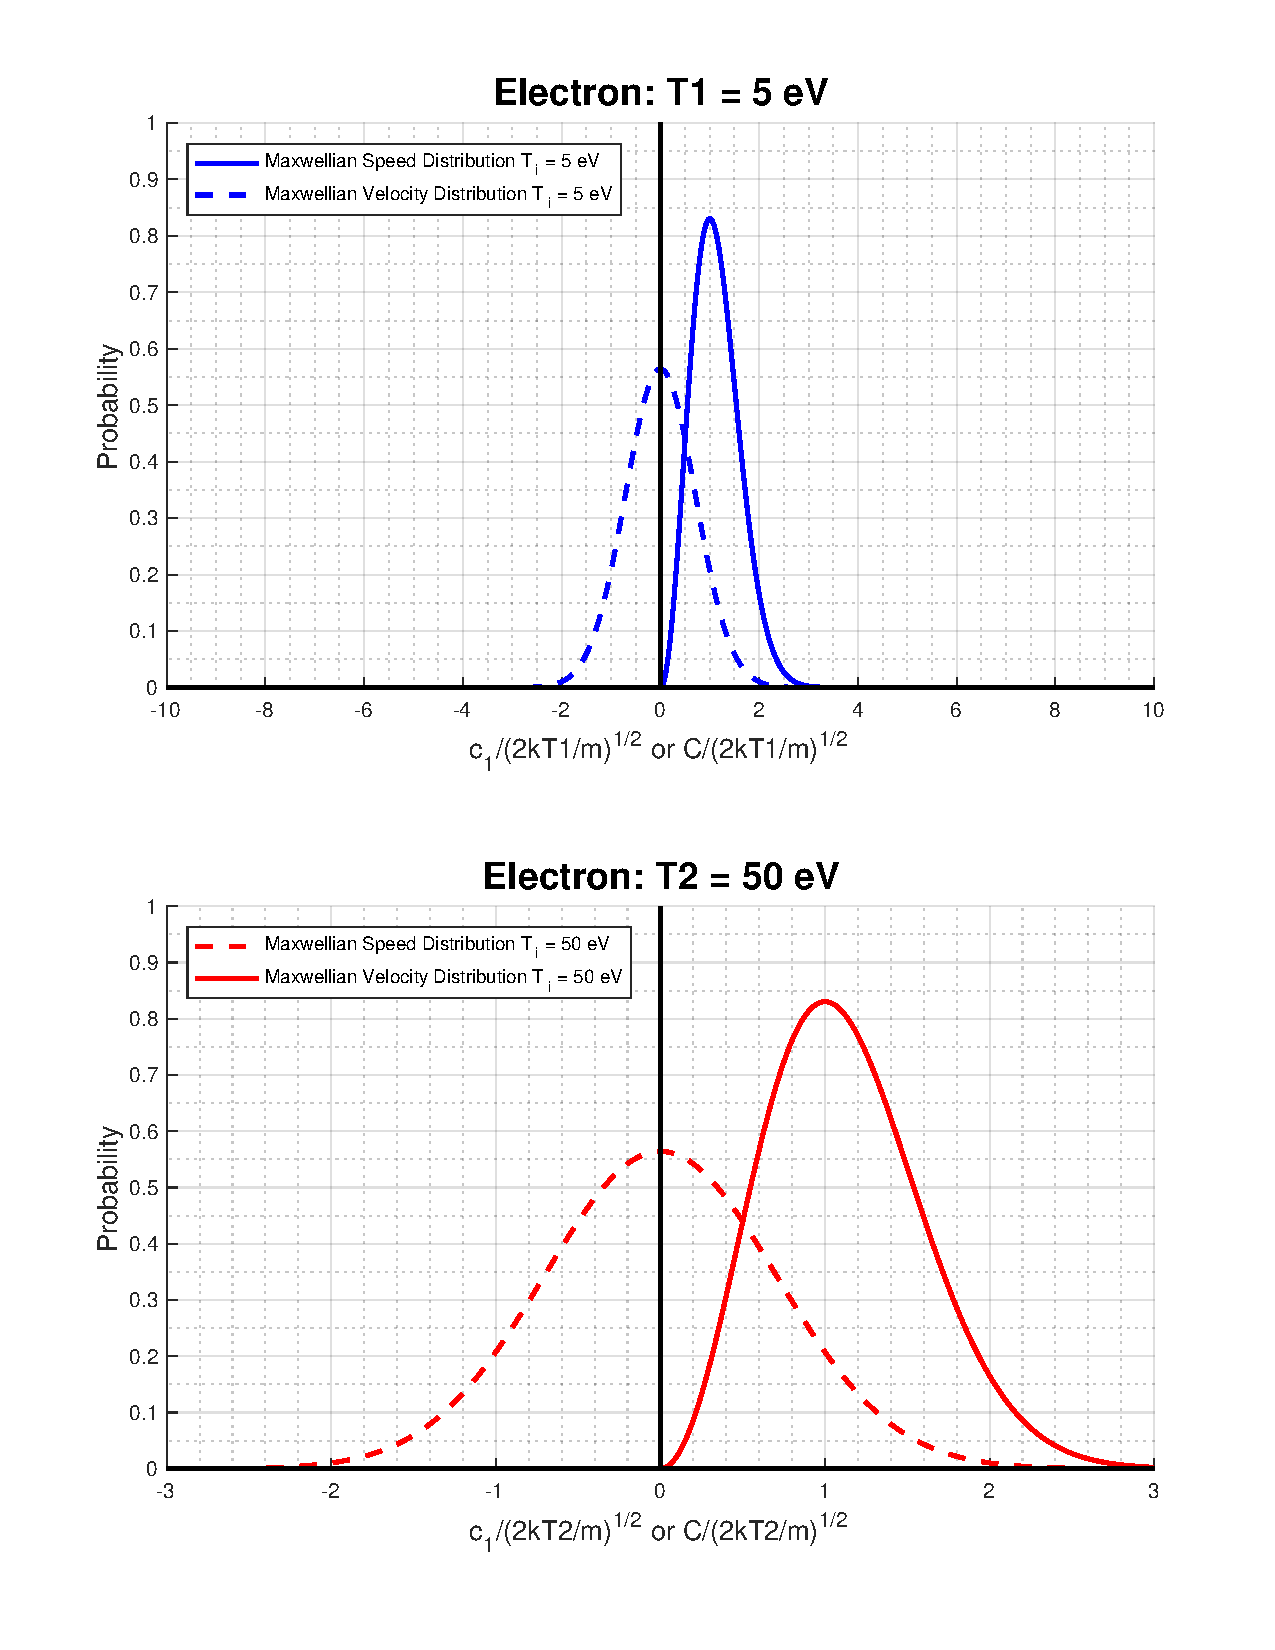
\includepdf{electronBothSubed.pdf}
\section*{Problem 3:Xenon}
\begin{figure}[H]
\begin{lstlisting}
clc; clear;

% Initialize variables
m = 2.18e-25;     % Mass of Xe Ion [kg]
k = 1.38e-23;     % Boltzmann's constant [J/K]
Te = [.5; 5];           % Particle Temperature [eV]

% Convert eV to K
T = 1.16045221e4*Te; %Temperature [K]

% Compute two frequently used constants
C1 = [4*pi*(m/(2*pi*k*T(1)))^(3/2);4*pi*(m/(2*pi*k*T(2)))^(3/2);]
C2 = [m/(2*k*T(1));m/(2*k*T(2))];
C3 = [(m/(2*pi*k*T(1)))^(1/2);(m/(2*pi*k*T(2)))^(1/2)];

c_mp1 = sqrt((2*k*T(1))/(m)) %Most Probable Speed
c_mp2 = sqrt((2*k*T(2))/(m))

c = [-3*c_mp2:50:3*c_mp2];  % Particle Velocity Magnitude [m/s]
for i=1:length(c)
    %Maxwellian Speed Distribution Function
    if c(i)<0
        chiM(1,i)=0;
        chiM(2,i)=0;
    else
        chiM(1,i) = C1(1) * c(i)^2 * exp(-C2(1) * c(i)^2);
        chiM(2,i) = C1(2) * c(i)^2 * exp(-C2(2) * c(i)^2);
    end
    
    %Maxwellian Velocity Distribution Function
    fM(1,i) = C3(1) * exp(-C2(1) * c(i)^2);
    fM(2,i) = C3(2) * exp(-C2(2) * c(i)^2);

end
hold on
plot(c/c_mp1,chiM(1,:)*c_mp1,'-b','LineWidth',2) %normalize with cmp.
plot(c/c_mp1,chiM(2,:)*c_mp1,'-r','LineWidth',2) %normalize with cmp.
plot(c/c_mp1,fM(1,:)*c_mp1,'--b','LineWidth',2)
plot(c/c_mp1,fM(2,:)*c_mp1,'--r','LineWidth',2)
hold off

subplot(2,1,1)
hold on
plot(c/c_mp1,chiM(1,:)*c_mp1,'-b','LineWidth',2) %normalize with cmp.
plot(c/c_mp1,fM(1,:)*c_mp1,'--b','LineWidth',2)

subplot(2,1,2)
hold on
plot(c/c_mp2,fM(2,:)*c_mp2,'--r','LineWidth',2)
plot(c/c_mp2,chiM(2,:)*c_mp2,'-r','LineWidth',2) %normalize with cmp.
\end{lstlisting}
\caption{Problem 3: Normalized Velocity and Speed Distribution Function Code for Xenon}
\end{figure}
\newpage
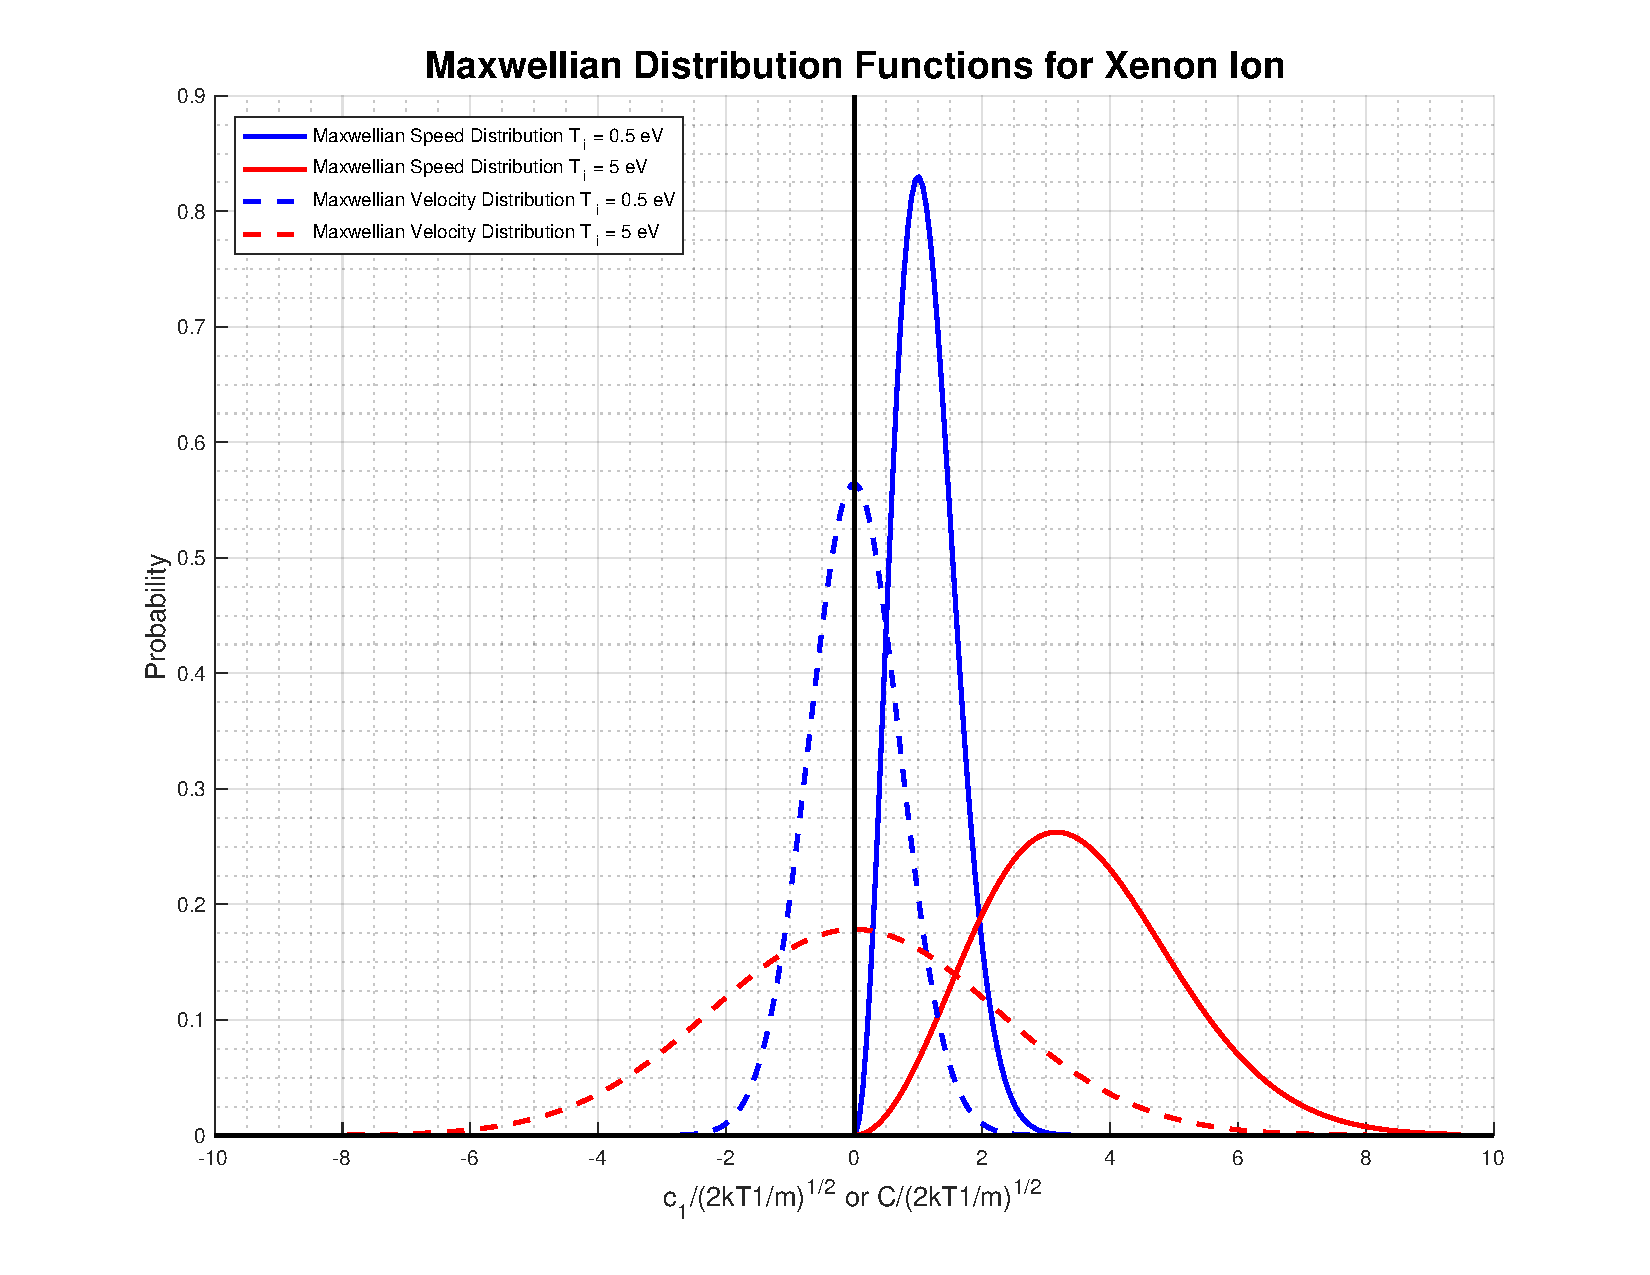
\includepdf{XeBoth.pdf}
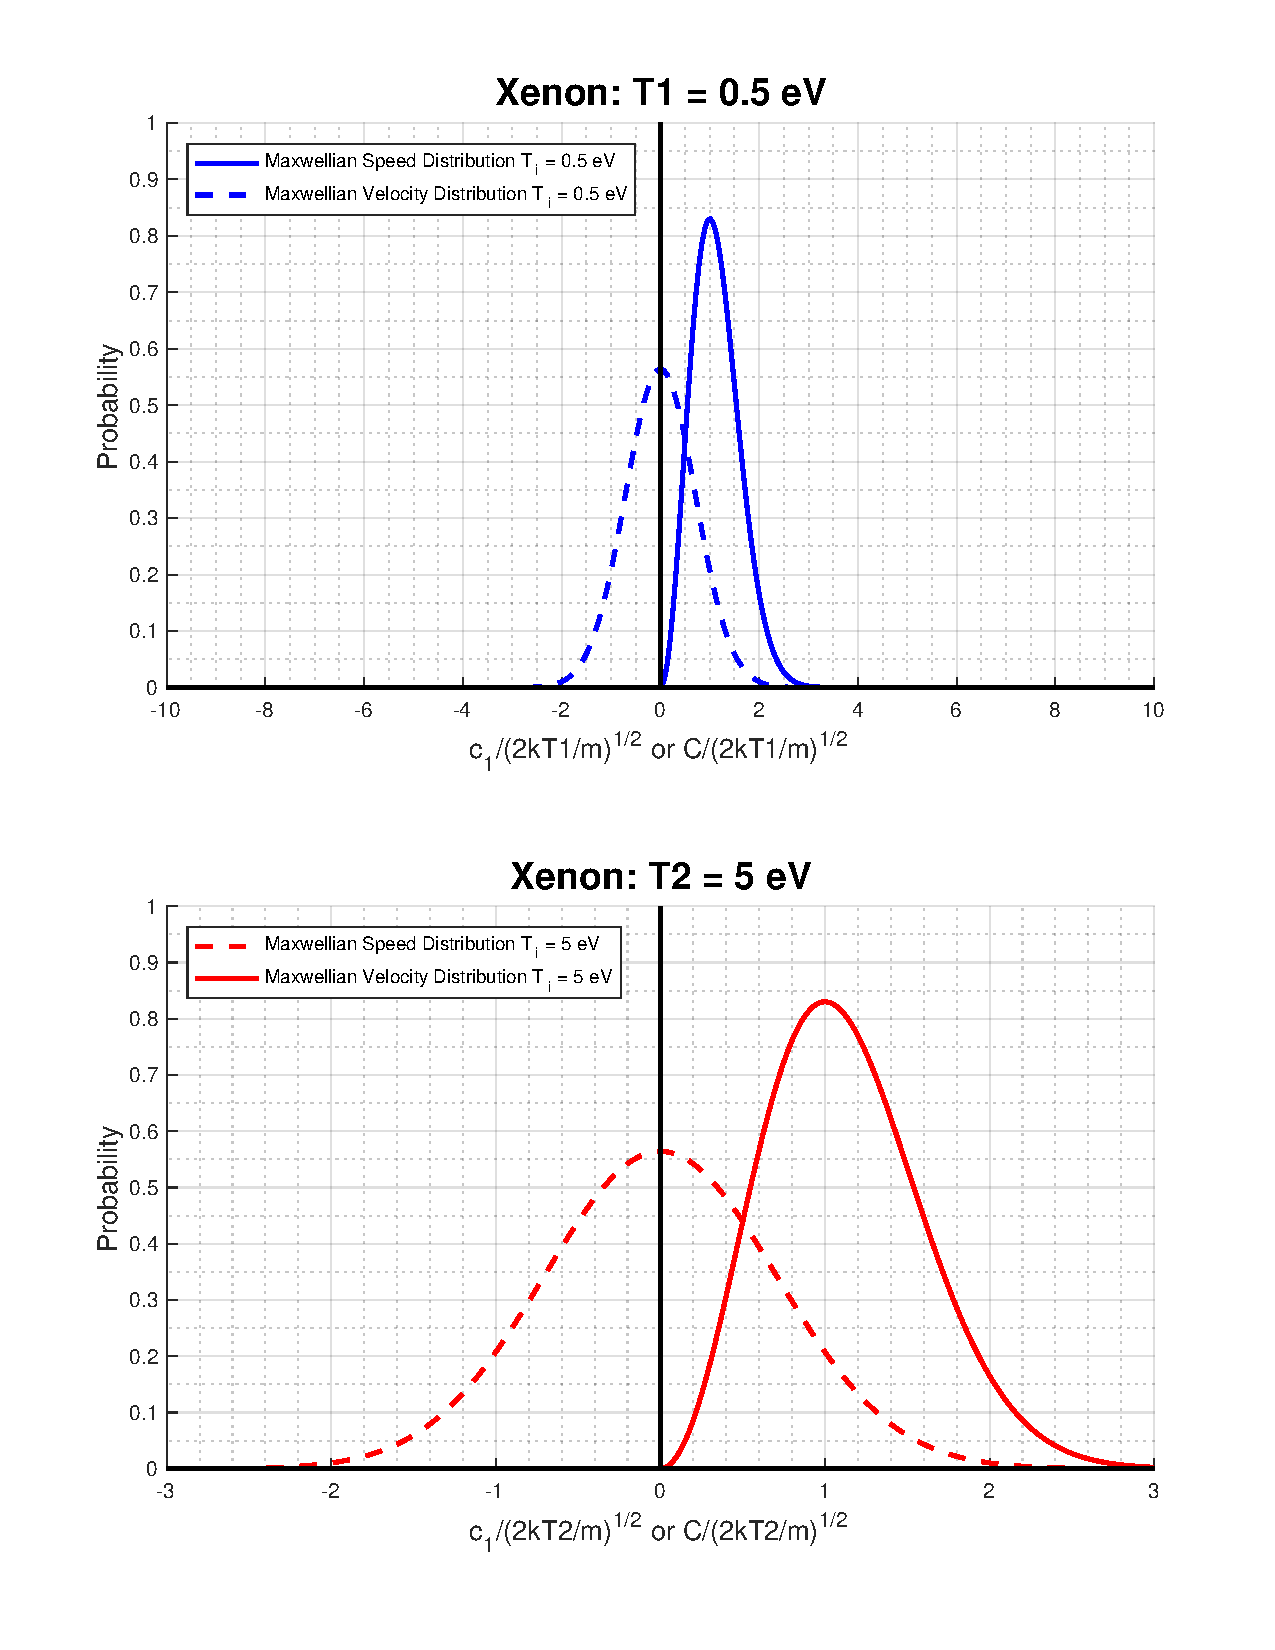
\includepdf{XeBothSubed.pdf}
\section*{Problem 3: Playground}
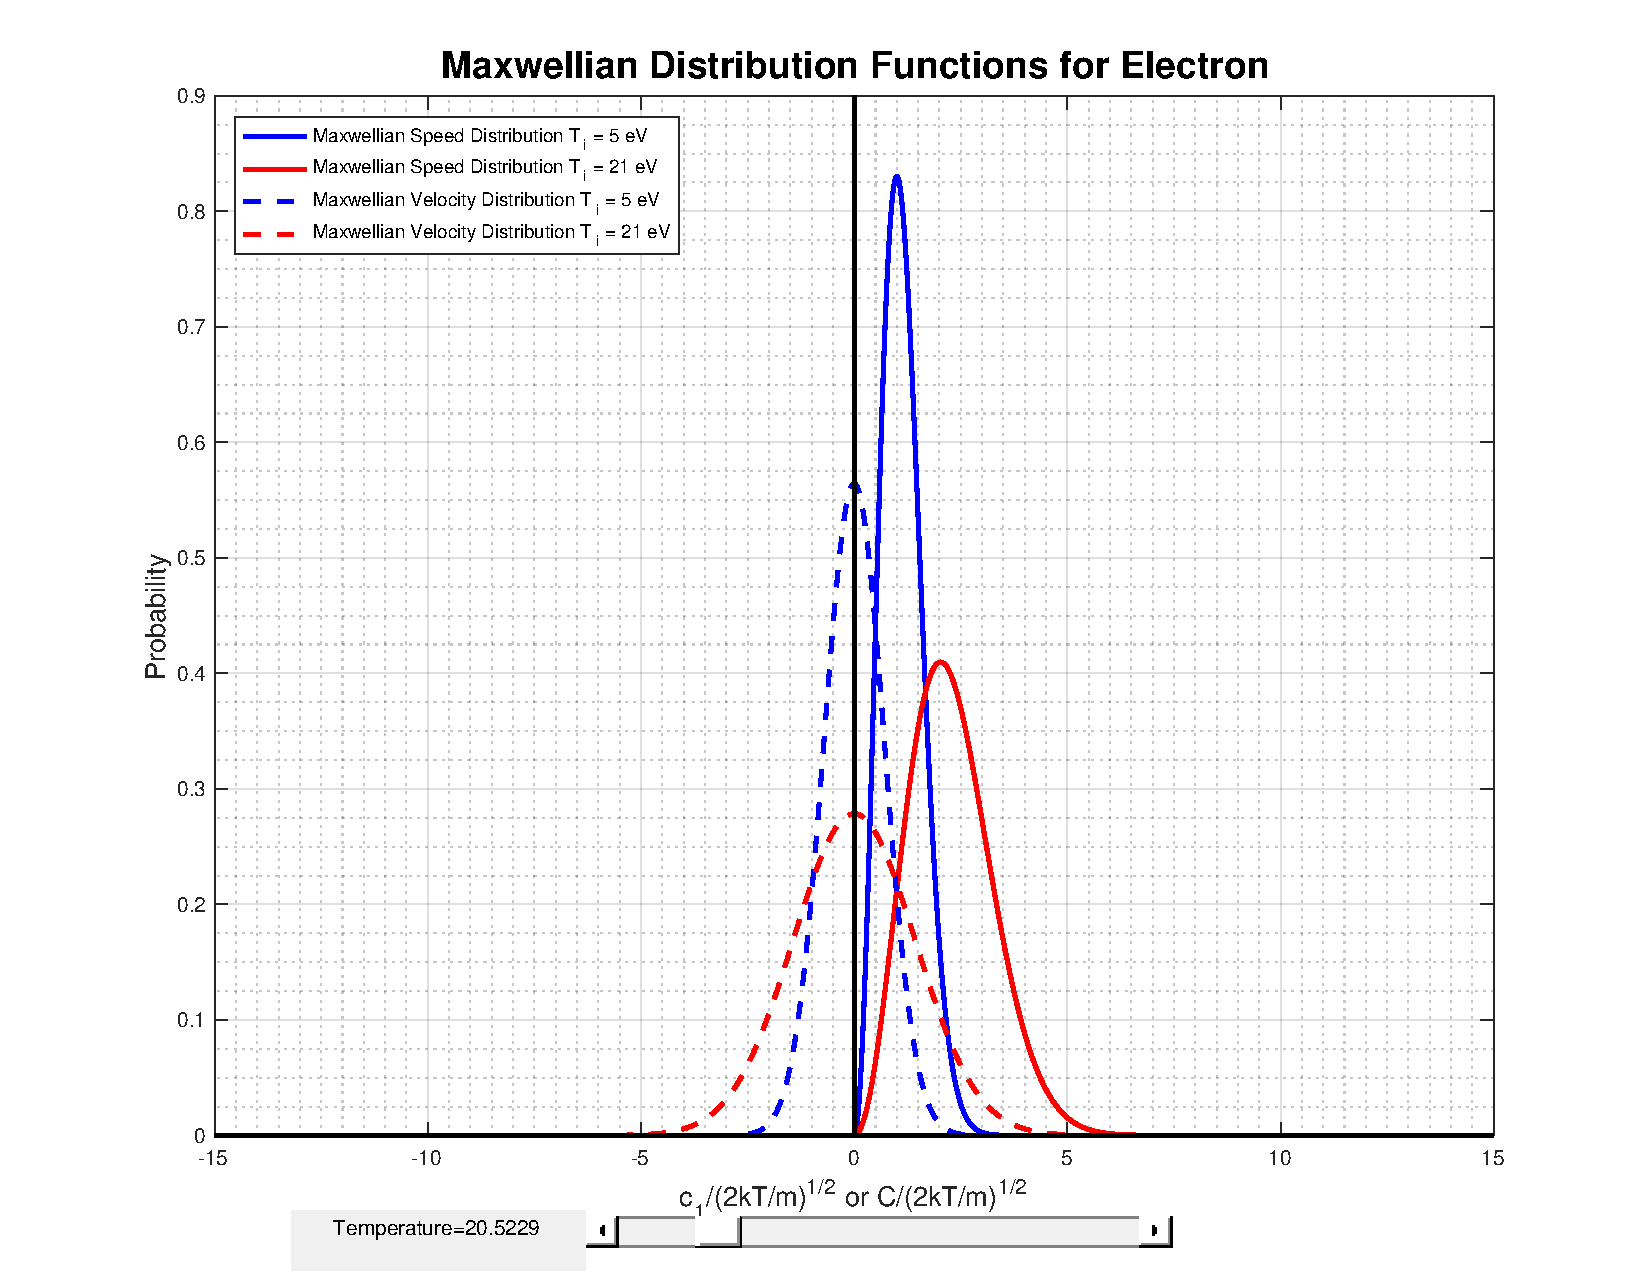
\includepdf{ElectronPlayground.pdf}
\section*{Problem 4:}
\begin{figure}[H]
\begin{lstlisting}
function hw4p4
    T = [2000:100:6000];
    P = [10^-3, 10^-1, 10];
    for i=1:length(T)
        AlphaPT(1,i)=SAHA(P(1),T(i));
        AlphaPT(2,i)=SAHA(P(2),T(i));
        AlphaPT(3,i)=SAHA(P(3),T(i));
    end
    plot(T,AlphaPT,'LineWidth',2)
    %Ploting code removed for space
    
    %Atomic Xenon Partition Function (AXPF)
    function f_A = AXPF(T)
        th = T/1; %Dimensionless Temperature T/To
        f_A = -1.08e-21*th^5 + 1.86e-16*th^4 -6.49e-12*th^3 + 8.97e-8*th^2 -5.42e-4*th + 2.02;
    end

    %Ionic Xenon Partition Function (IXPF)
    function f_p = IXPF(T)
        th = T/1; %Dimensionless Temperature T/To
        f_p = 5.8e-17*th^4 -3.71e-12*th^3 + 8.0e-8*th^2 -6.37e-4*th + 6.97;
    end

    %SAHA Equation
    function alpha = SAHA(P,T)
        m = 2.18e-25; %Mass of Xenon [kg]
        k = 1.38e-23; % Boltzmann's constant [J/K]
        h = 6.62607e-34;%Planck's Constant [m^2 kg/s]
        epsilon_i = 12.13; %Ionization Energy wrt. Atomic Ground State [eV]
        epsilon = 1.60218e-19*epsilon_i; %Ionization Energy [J]
        
        P = P*133.322; %torr to Pa [kg/ m s^2]
        syms alpha real
        term1 = ((2*((2*pi*m)^(3/2))*((k*T)^(5/2)))/(P*h^3));
        term2 = (IXPF(T)/AXPF(T));
        term3 = exp(-epsilon/(k*T));
        eqn1 = ((alpha^2)/(1-alpha^2)) == term1*term2*term3;
        sol = vpa(solve(eqn1, alpha));
        alpha = sol(2);
    end
end

\end{lstlisting}
\caption{Problem 4: Ionization for Xenon with Dependence on Pressure and Temperature}
\end{figure}
\newpage
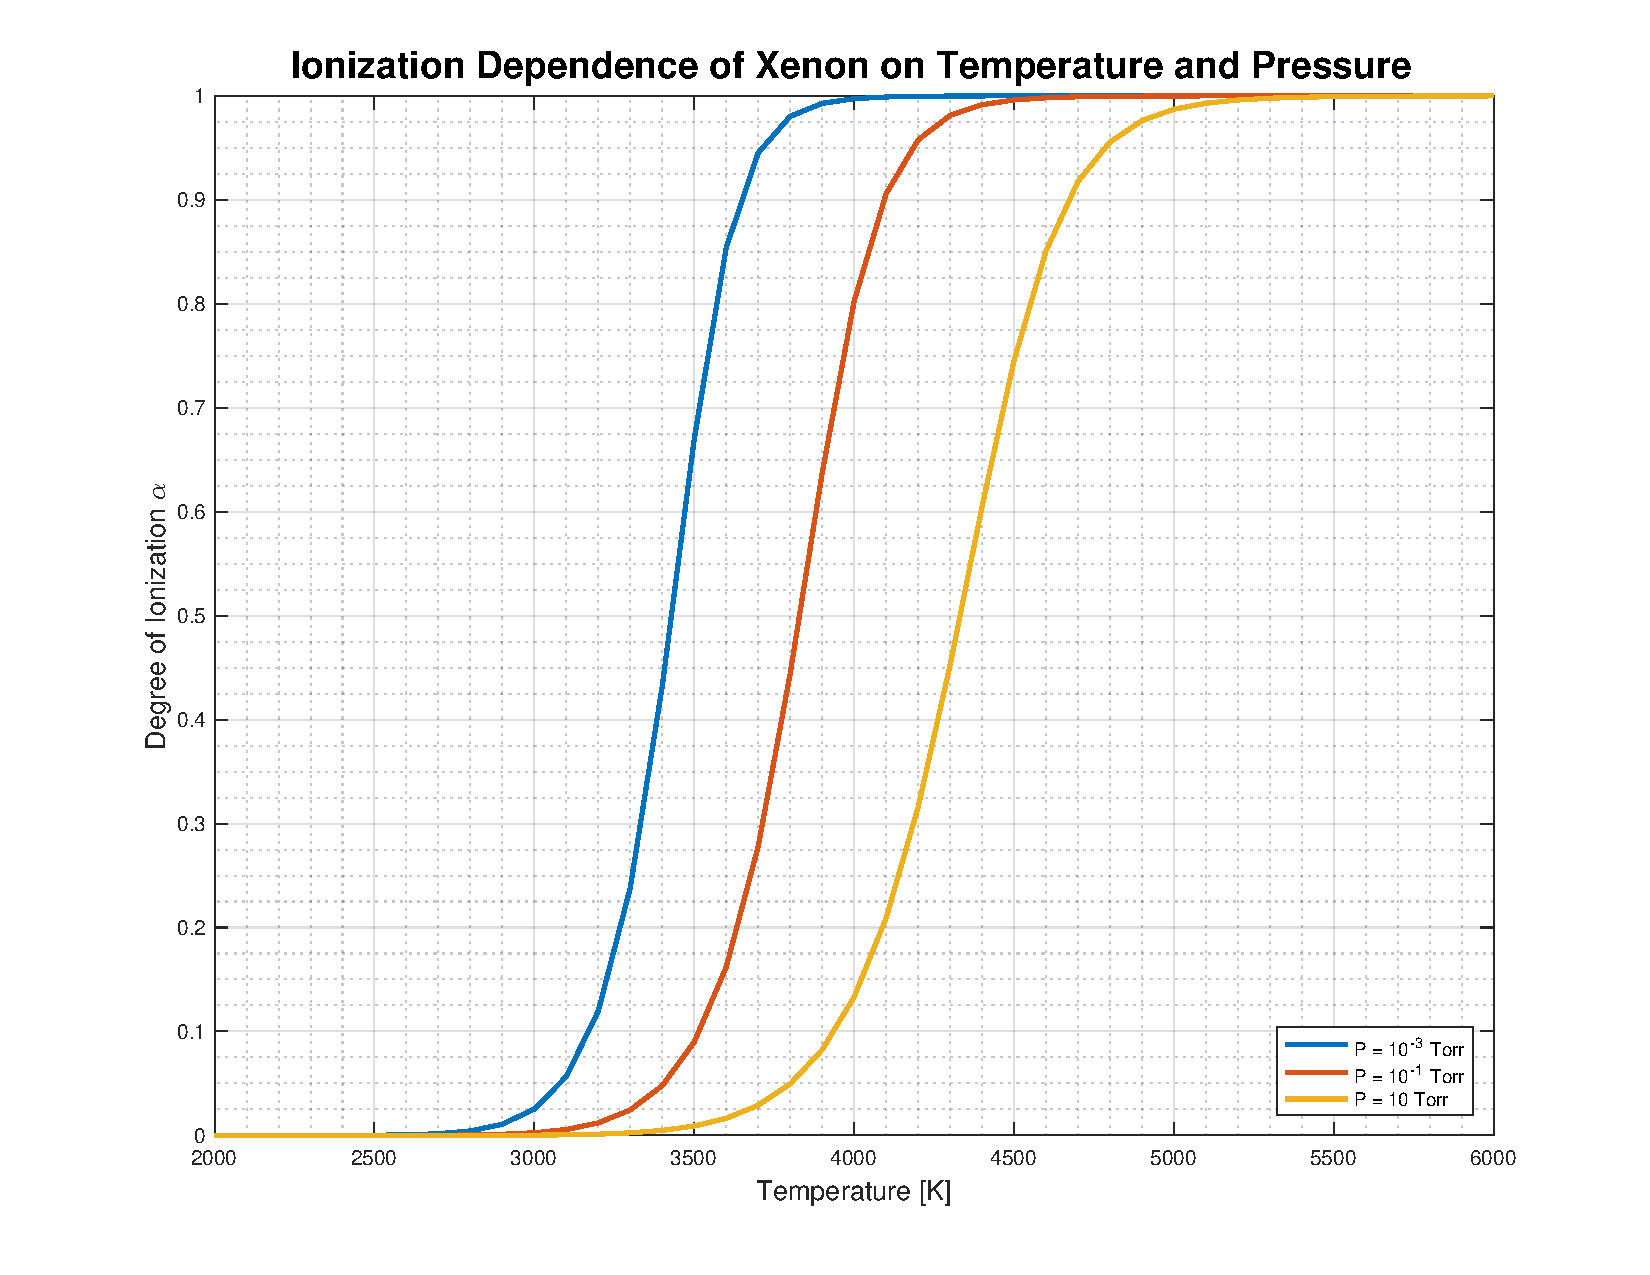
\includepdf{p4.pdf}

\end{document}